% =================================================================================================
% File:			riassunto_riunione.tex
% Description:	Defiinisce la sezione relativa a ...
% Created:		2015-02-19
% Author:		Cusinato Giacomo
% Email:		cusinato.giacomo@mashup-unipd.it
% =================================================================================================
% Modification History:
% Version		Modifier Date		Change											Author
% 0.0.1 		2015-02-19 			stesura riassunto della riunione				Cusinato Giacomo
% =================================================================================================
%

% CONTENUTO DEL CAPITOLO

\section{Riassunto della riunione} % (fold)
\label{sec:riassunto_della_riunione}

\subsection{Risposte all'ordine del giono}
Le risposte di seguito fornite non sono la trascrizione esatta di quanto detto al momento, ma una
elaborazione finale in accordo con il proponente.
\begin{itemize}
  \item La struttura del sistema ha subito delle modifiche che rendono l'applicativo più efficente
  per il suo funzionamento nella Google Cloud Platform. Si è deciso infatti che ogni modulo che
  interrogherà una certa API sarà inserito in una piattaforma web differente (Google App Engine differente).
  Questi moduli conterranno a sua volta un modulo Miner, un modulo Processor, un Cron e un Database NoSQL
  come in precedenza. In questo modo, oltre a distrubuire il carico di lavoro che può causare il superamento
  della soglia gratuita del servizio, ogni modulo risulterà più estensibile essendo indipendente dagli altri;

  \item Con l'aiuto del proponente sono state discusse le prime analisi effettuate sulla ricerca della
  tipologia di dati da ricavare tramite le API esposte dai vari social network. In particolar modo, sono
  state indivuduate le prime metriche che andranno a definire le funzionalità rese disponibili dalle View e
  che individueranno i dati grezzi necessari alle Recipe;

  \item Il proponente ha fornito un elenco di servizi web che potrebbero facilitare l'analisi dei dati
  ricavati dai social network o, in alcuni casi, fornire funzionalità ed informazioni aggiuntive al
  risultato finale esposto dalle View, grazie alle API esposte da ognuno di essi. Tali servizi sono:
  \begin{itemize}
    \item \textbf{PageSpeed Insights}: servizio fornito da Google per l'analisi della velocità ed il
    rendimento di un sito web;
    \item \textbf{MozRank}: fornisce informazioni sull'importanza di un sito web a seconda della qualità
    pagine che contengono uno o più link a tale sito;
    \item \textbf{Feedly}: espone delle API che forniscono dati e statistiche sull'uso dei feed all'interno
    del servizio, inclusi topic, categorie, tag ed interessi popolari tra gli utenti;
    \item \textbf{Ritetag}: fornisce analisi e statistiche sul trend e la popolarità di determinati hashtag;
    \item \textbf{Klout}: fornisce analisi sull'influenza generata da parte di una pagina o di un profilo
    attivo in un social network;
    \item \textbf{ShareCount}: traccia l'andamento di un URL nei vari social network;
    \item \textbf{W3C}: fornisce errori sul codice front-end di un determinato sito web;
    \item \textbf{GTMetrix}: fornisce analisi sulla pesantezza e la velocità di una pagina web.
  \end{itemize}
\end{itemize}

\subsection{Specifica sui moduli individuati}

\begin{figure}[htbp]
    \centering
    \centerline{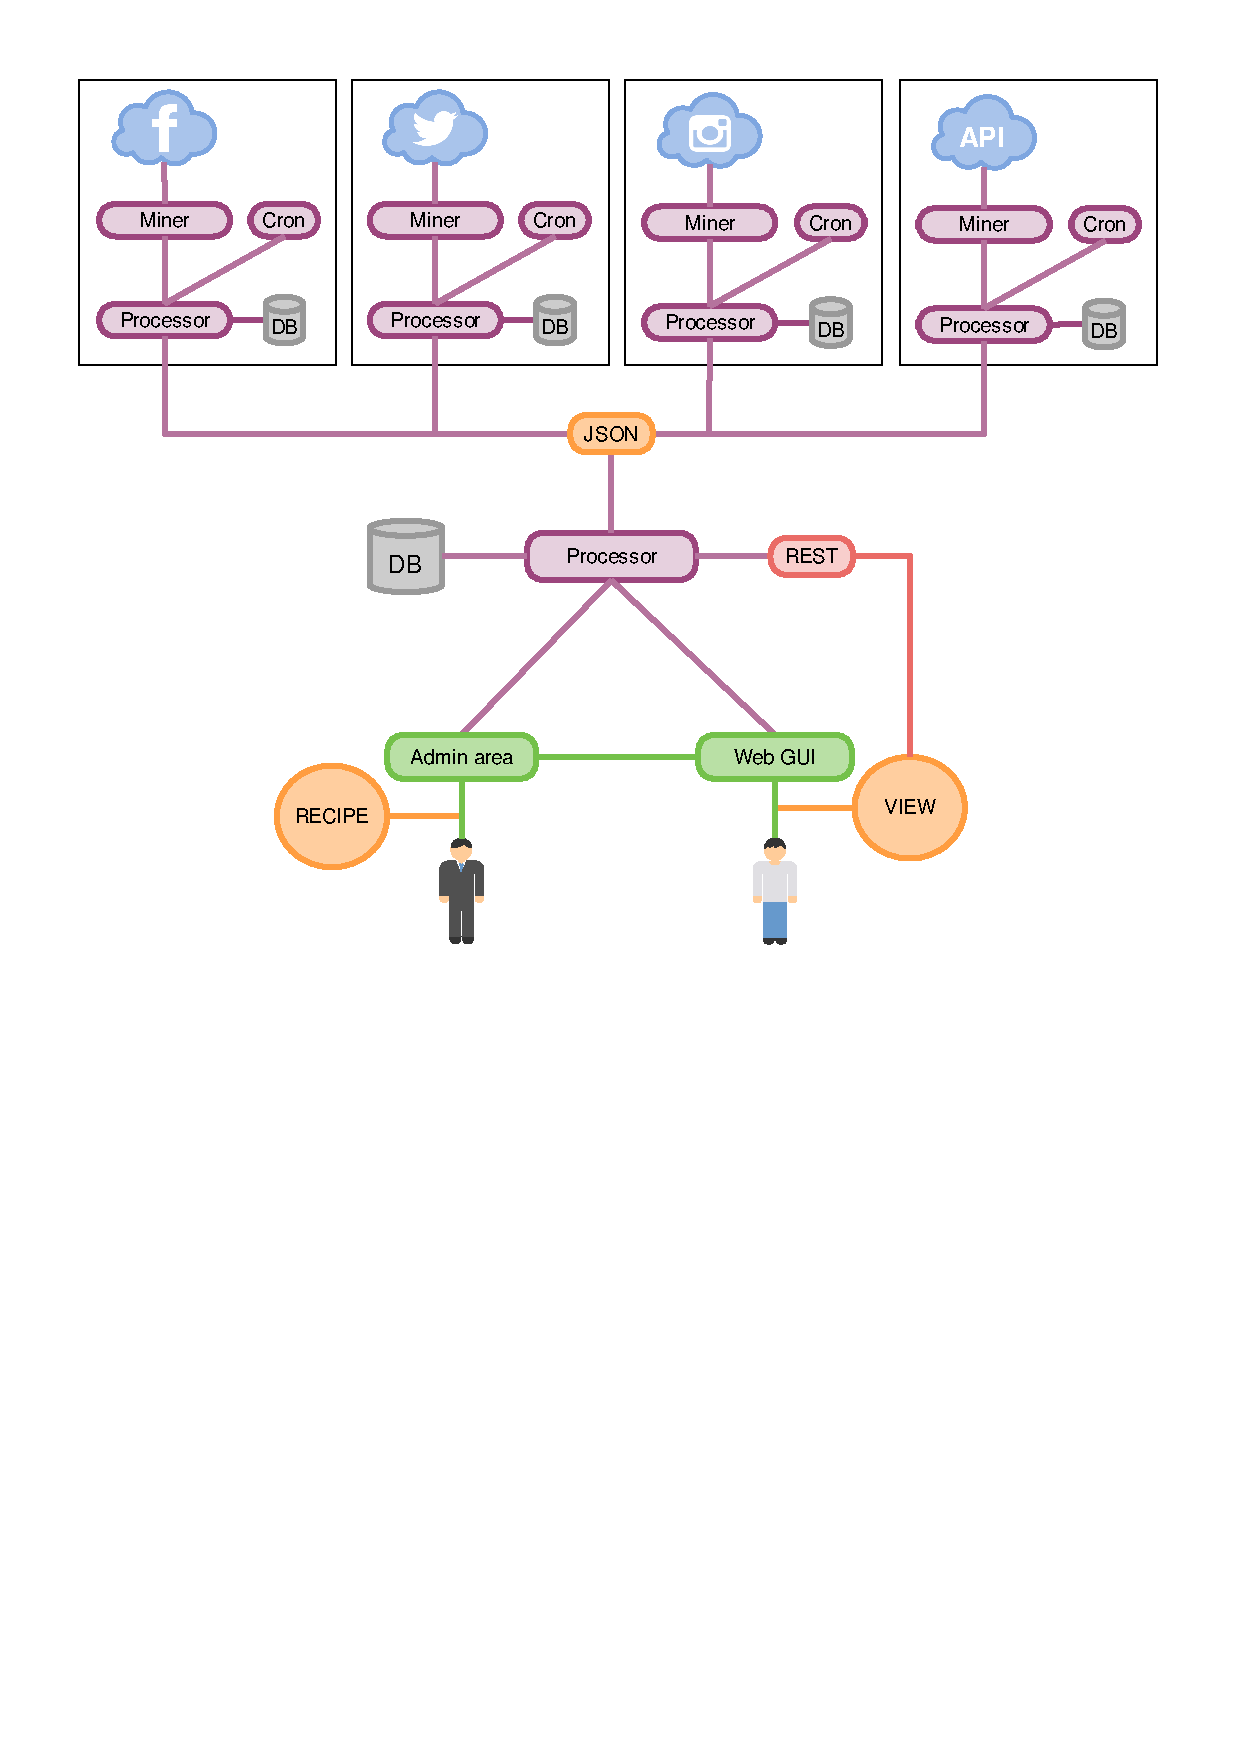
\includegraphics[scale=0.8]{./images/moduli_bdsmapp.pdf}}
    \caption{Moduli applicativo}
\end{figure}

La struttura dell'applicativo è stata aggiornata in modo tale da distribuire lo spazio riservato al database
ed il carico di lavoro affidato al sistema. Ogni modulo responsabile di ricavare i dati da un determinato
social network sarà infatti inserito in un'infrastruttura differente che richiederà la creazione di più accout
nella piattaforma di Google. Ogni modulo, quindi, conterrà la struttura Miner, Cron e Processor stabilita in
precedenza ed un database NoSQL che conterrà i dati grezzi. Il vantaggio di questa soluzione è data dal fatto
che ogni modulo risulta indipendente dai restanti e potrà essere progettato in modo specifico per le funzionalità
che dovrà fornire. Inoltre, sebbene la possibilità di superamento della soglia gratuita del servizio offerto da
Google non dovrebbe causare problemi, la distribuzione del sistema su più account renderà tale problematica meno
rilevante.
Tutti i moduli saranno gestiti da un Processor centrale, il quale, interagirà con un database NoSQL principale che
memorizzerà i dati di configurazione dell'applicativo ed i riferimenti ai dati dei database secodari di ogni modulo
sopracitato. Il Processor centrale, inoltre, si occuperà di elaborare i dati grezzi ed esporli alla WebGUI
tramite dei servizi di tipo REST.
